\section{Introdução}\label{introduuxe7uxe3o}

O aplicativo Wireless Monitor tem o objetivo de permitir que um
desenvolvedor de sistemas embarcados possam enviar para a nuvem os dados
obtidos por seu equipamento IOT e visualizá-los no navegador.

\section{Objetivos}\label{objetivos}

A ideia principal é criar uma \emph{api} leve e simples, visto que
equipamentos IOT são limitados. Tendo isso em vista, vejamos os passos
para criar um projeto.

\subsection{Cadastro do desenvolvedor}\label{cadastro-do-desenvolvedor}

O desenvolvedor inicialmente deve fazer um cadastro simples na
ferramenta. Esse cadastro irá criar para ele uma \texttt{api\_key}, ou
seja, uma chave única no formato UUIDv4.

\subsection{Criar um \emph{Monitor}}\label{criar-um-monitor}

Um \emph{Monitor} é um componente interno do sistema criado pelo
desenvolvedor de acordo com sua necessidade, é o instrumento que
caracteriza os dados coletados e os apresenta na interface web.

Imagine que o desenvolvedor queira medir a temperatura de um ambiente e
acompanhar suas variações. Para isso ele deve criar um \emph{Monitor} de
Temperatura, que apenas recebe um valor a um certo intervalo de tempo.
Dessa forma o desenvolvedor pode acompanhar as variações ou ainda ver em
forma de gráfico um conjunto de variações de um período de tempo
anterior.

Da mesma forma que uma chave UUID é criada para o desenvolvedor, uma
chave é criada para o Monitor - \texttt{monitor\_key}.

\subsection{Autenticação do
equipamento}\label{autenticauxe7uxe3o-do-equipamento}

Para autenticar e identificar o desenvolvedor e seu \emph{monitor} é
preciso enviar a \texttt{api\_key} e a \texttt{monitor\_key} via método
\emph{POST} para o \emph{endpoint} \texttt{/api/authenticate}. Em caso
positivo o sistema irá retornar um \emph{token}. Esse \emph{token}
servirá para qualquer troca de informações futuras entre o equipamento
IOT e o sistema. Esse método de autenticação é chamado de JWT ou
\emph{JSON Web Token}, um padrão internacional \emph{RFC 7519} para
intercâmbio de dados entre entidades.

Após ter o \emph{token} o desenvolvedor deve passá-lo através da
\emph{Header HTTP} denominada \emph{Authorization} usando \emph{schema
Bearer}. Algo do tipo:

\begin{verbatim}
Authorization: Bearer <token>
\end{verbatim}

Um \emph{token} é formado pelas seguintes informações:

\begin{itemize}
\itemsep1pt\parskip0pt\parsep0pt
\item
  \emph{Header}
\item
  \emph{Payload}
\item
  \emph{Signature}
\end{itemize}

Essa é uma forma segura e com pouco custo de memória. Além de ser uma
forma de autenticação \emph{stateless}, em que não são usadas sessões e
nem mesmo \emph{cookies}.

\subsection{Envio dos dados}\label{envio-dos-dados}

Além do cabeçalho contendo o \emph{token} o usuário deve passar os
valores coletados pelo equipamento e enviar para o sistema. Para isso
ele deve enviar uma requisição \emph{POST} para o \emph{endpoint}
\texttt{/api/send}, com o atributo \texttt{data} contendo um JSON com os
dados.

No exemplo do \emph{Monitor} de temperatura é necessário enviar apenas o
valor, algo do tipo:

\begin{verbatim}
{
    "value": 23.89
}
\end{verbatim}

Sumarizando o código final seria algo como:

\begin{verbatim}
HTTPClient http;
http.begin("https://wireless-monitor.site/api/send");
http.addHeader("Content-Type", "application/json");
http.addHeader("Authorization", "Bearer <token>");
http.POST("data={value:23.89}");
http.writeToStream(&Serial);
http.end();
\end{verbatim}

\subsection{Visualização dos dados}\label{visualizauxe7uxe3o-dos-dados}

Após captar e enviar dados do IOT para a nuvem é possível acompanhar os
resultados pelo sistema. A forma de visualização será como mostra a
Figura \ref{fig:view-monitor}

\begin{figure}[h]
    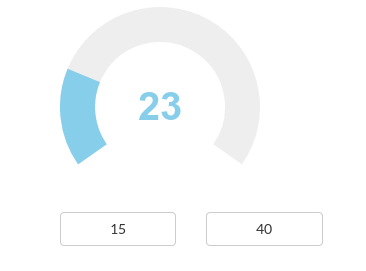
\includegraphics[scale=0.5]{img/wm-monitor-temperature.png}
    \caption{Visualização dos dados na web} \label{fig:view-monitor}
\end{figure}

\section{Cronograma}\label{cronograma}

\begin{longtable}[c]{@{}lllll@{}}
\toprule\addlinespace
\begin{minipage}[b]{0.39\columnwidth}\raggedright
Tarefas
\end{minipage} & \begin{minipage}[b]{0.12\columnwidth}\raggedright
Semana 1
\end{minipage} & \begin{minipage}[b]{0.12\columnwidth}\raggedright
Semana 2
\end{minipage} & \begin{minipage}[b]{0.12\columnwidth}\raggedright
Semana 3
\end{minipage} & \begin{minipage}[b]{0.12\columnwidth}\raggedright
Semana 4
\end{minipage}
\\\addlinespace
\midrule\endhead
\begin{minipage}[t]{0.39\columnwidth}\raggedright
Protótipo Inicial
\end{minipage} & \begin{minipage}[t]{0.12\columnwidth}\raggedright
X
\end{minipage} & \begin{minipage}[t]{0.12\columnwidth}\raggedright
\end{minipage} & \begin{minipage}[t]{0.12\columnwidth}\raggedright
\end{minipage} & \begin{minipage}[t]{0.12\columnwidth}\raggedright
\end{minipage}
\\\addlinespace
\begin{minipage}[t]{0.39\columnwidth}\raggedright
Programação
\end{minipage} & \begin{minipage}[t]{0.12\columnwidth}\raggedright
X
\end{minipage} & \begin{minipage}[t]{0.12\columnwidth}\raggedright
X
\end{minipage} & \begin{minipage}[t]{0.12\columnwidth}\raggedright
X
\end{minipage} & \begin{minipage}[t]{0.12\columnwidth}\raggedright
\end{minipage}
\\\addlinespace
\begin{minipage}[t]{0.39\columnwidth}\raggedright
Testes
\end{minipage} & \begin{minipage}[t]{0.12\columnwidth}\raggedright
\end{minipage} & \begin{minipage}[t]{0.12\columnwidth}\raggedright
\end{minipage} & \begin{minipage}[t]{0.12\columnwidth}\raggedright
X
\end{minipage} & \begin{minipage}[t]{0.12\columnwidth}\raggedright
X
\end{minipage}
\\\addlinespace
\begin{minipage}[t]{0.39\columnwidth}\raggedright
Relatório
\end{minipage} & \begin{minipage}[t]{0.12\columnwidth}\raggedright
X
\end{minipage} & \begin{minipage}[t]{0.12\columnwidth}\raggedright
\end{minipage} & \begin{minipage}[t]{0.12\columnwidth}\raggedright
\end{minipage} & \begin{minipage}[t]{0.12\columnwidth}\raggedright
X
\end{minipage}
\\\addlinespace
\bottomrule
\addlinespace
\caption{Cronograma}
\end{longtable}
